Let \lstinline'a' and \lstinline'b' be linked lists with $m$ and $n$
data values in them, respectively. For each of the pictures below,
draw the final state of the lists after \lstinline'mystery(a,b)'
executes.
\part[1\half]\hfill\rule{0em}{0ex}\TAGS{linked-list, testing}
\begin{center}
\vspace*{-3ex}%
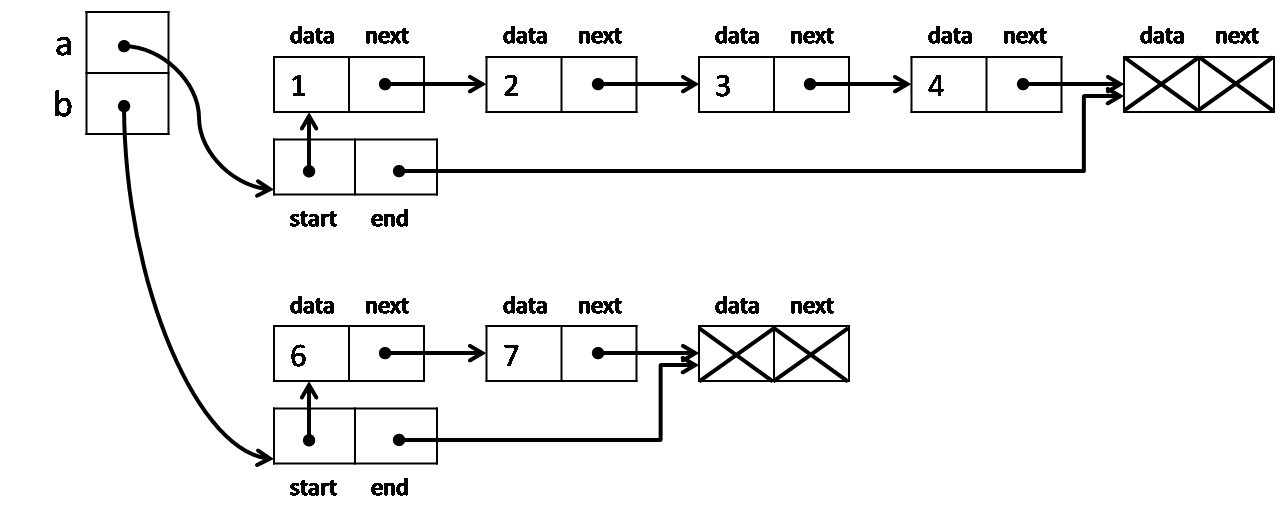
\includegraphics[scale=0.55]{\img/linked1.png}
\end{center}
\vspace*{-2ex}%
\begin{framed}
\ifprintanswers{\color{\answerColor}
  a: 1->6->2->7->3->4->X

  \medskip
  b: X
}\else~\vspace{1.5in}\fi
\end{framed}


\bigskip
\begin{center}
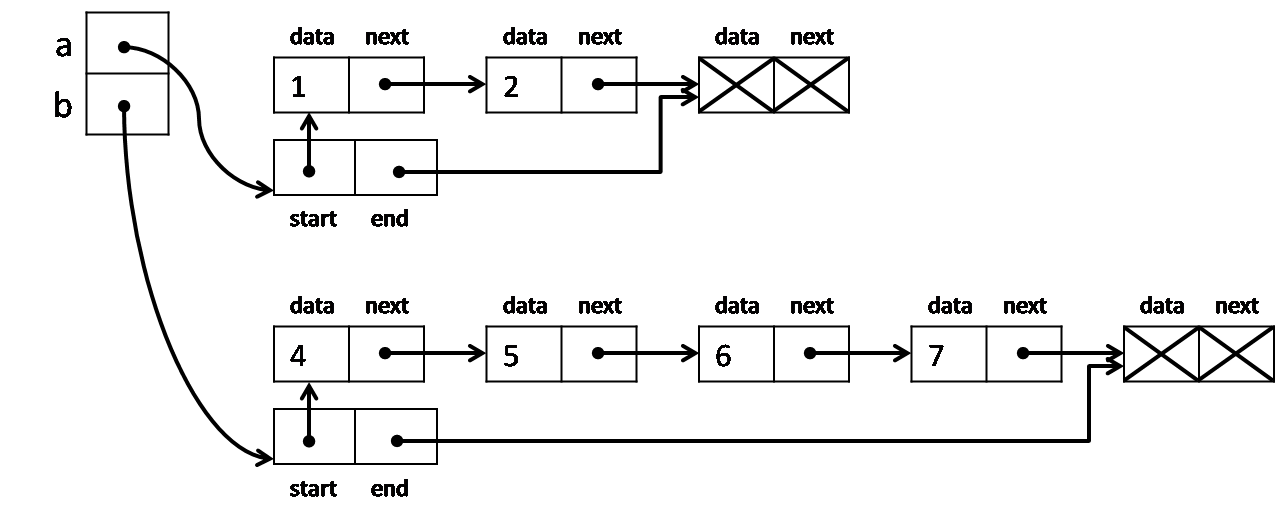
\includegraphics[scale=0.55]{\img/linked2.png}
\end{center}
\vspace*{-2ex}%
\begin{framed}
\ifprintanswers{\color{\answerColor}
  a: 1->4->2->5->X

  \medskip
  b: 6->7->X
}\else~\vspace{1.5in}\fi
\end{framed}

\enlargethispage{5ex}
\medskip
What is the final length of linked list \lstinline'a' when

\noindent
\begin{minipage}[t]{0.45\linewidth}
  \centering $\bullet \quad m \ge n$
  \begin{framed}
    \medskip
    \answer{14em}{$m+n$}
  \end{framed}
\end{minipage}
\hfill
\begin{minipage}[t]{0.45\linewidth}
\centering $\bullet \quad m < n$
  \begin{framed}
    \medskip
    \answer{14em}{$2m$}
  \end{framed}
\end{minipage}

\RUBRIC
Part (c)
TAGS: linked-list, testing

Gradescope rubric:
+0.15pt: a and b are two distinct lists, both of which are valid
+0.35pt: EITHER box 1 contains a: 1->6->2->7->3->4->X,  b: X
+0.15pt: OR    box 1 has at most one pair of mistakes

+0.15pt: a and b are two distinct lists, both of which are valid
+0.35pt: EITHER box 2 contains a: 1->4->2->5->X, b: 6->7->X
+0.15pt: OR    box 2 has at most one pair of mistakes

+0.25pt: First box: m+n
+0.25pt: Second box: 2m
-0.1pt:  Off by one on either
Commentary: (none)

ENDRUBRIC
